\documentclass{pre-tfg}

\usepackage{listings}
\usepackage{formular}
\usepackage{listings}
\usepackage[pdftex]{graphicx}
\usepackage{caption}
\usepackage{subcaption}

%\showhelp  % comenta o borra para eliminar ayudas

\title{COMPARADOR DE CONFIGURACIONES DE ORDENADOR POR COMPONENTES}
\author{Álvaro Ángel-Moreno Pinilla y Carlos Córdoba Ruiz}
\advisorFirst{Luis Rodriguez Benitez}
\advisorDepartment{DEPARTAMENTO DE TECNOLOGÍAS Y SISTEMAS DE INFORMACIÓN}
\advisorSecond{}
\intensification{COMPUTACIÓN}
\docdate{2018}{14 Enero}

\DeclareGraphicsExtensions{.pdf,.png,.jpg}

\usepackage{color}
\definecolor{gray97}{gray}{.97}
\definecolor{gray75}{gray}{.75}
\definecolor{gray45}{gray}{.45}

\lstset{ frame=Ltb,
     framerule=0pt,
     aboveskip=0.5cm,
     framextopmargin=3pt,
     framexbottommargin=3pt,
     framexleftmargin=0.4cm,
     framesep=0pt,
     rulesep=.4pt,
     backgroundcolor=\color{gray97},
     rulesepcolor=\color{black},
     %
     stringstyle=\ttfamily,
     showstringspaces = false,
     basicstyle=\small\ttfamily,
     commentstyle=\color{gray45},
     keywordstyle=\bfseries,
     %
     numbers=left,
     numbersep=15pt,
     numberstyle=\tiny,
     numberfirstline = false,
     breaklines=true,
   }

% minimizar fragmentado de listados
\lstnewenvironment{listing}[1][]
   {\lstset{#1}\pagebreak[0]}{\pagebreak[0]}

\lstdefinestyle{consola}
   {basicstyle=\scriptsize\bf\ttfamily,
    backgroundcolor=\color{gray75},
   }

\lstdefinestyle{C}
   {language=C,
   }


\renewcommand*\lstlistingname{Listado}



\begin{document}

\maketitle
\tableofcontents

\newpage

\section{DEFINICIÓN DEL PROBLEMA}
La idea de nuestro sistema surge en las compras on-line, donde varias páginas independientes ofrecen un mismo producto con determinados precios y ofertas. En un principio, el comparador estaría orientado a ser multiproducto, en gran diversidad de páginas web. En nuestro caso, para acotar más el problema, nos centramos en los componentes de ordenador y páginas web destinadas para ello. Bajo esas condiciones, la idea principal de nuestro sistema consiste en tomar el modelo de un producto como input, para así buscarlo en las páginas web de venta de componentes que definamos. Acto seguido, comparar los precios y la disponibilidad de cada una de las ofertas para así obtener una decisión sobre qué sitio web elegir para su compra.

Las herramientas que van a ser utilizada son:
	\begin{itemize}
		\item JADE: Entorno software que simplifica la comunicación entre los agentes del sistema (middleware).
		\item Jsoup: Librería de Java que permite trabajar con el código HTML de las páginas web a consultar.
		\item regex: Librería de Java que actúa como reconocedor de patrones, utilizado para obtener las características de cualquier producto en los sitios web.
	\end{itemize}

\section{ANTECEDENTES}
Actualmente existen numerosos servicios web que actúan mediante sistemas multiagente a modo de comparador. Entre ellos, se encuentran páginas como www.rastreator.com, un comparador de multiproducto de telefonía, viajes, finanzas y seguros. También cabe destacar www.acierto.com, comparador de seguros con los precios y coberturas de más de 30 compañías distintas.

Sin embargo, a pesar de la amplitud de productos que ambos ejemplos presentan, ninguno de ellos ofrece sus servicios en productos de ésta índole. Es por ello que podemos definir nuestra propuesta de sistema multiagente como una idea viable en la que trabajar.

\section{SITIOS WEB A CONSULTAR}
Existe una amplia diversidad de tiendas on-line que pueden vender un producto determinado, pero nuestro objetivo, acotado a componentes de ordenador, nos indica tomar páginas web más generalizadas dentro de la propia especificación electrónica. En dichos sitios web, la situación idónea es que se presenten una multitud de productos similares no sólo en características sino en el propio modelo del producto. Así, la meta de comparador sería la más  veraz y natural posible. Los dominios web en los que hemos elegido establecer nuestras comparaciones son:
\begin{itemize}
 	\item www.pccomponentes.com
	\item www.aussar.es
	\item www.newhomepc.net
\end{itemize}

\section{AGENTES Y COMPORTAMIENTOS}
El sistema final está formado por dos agentes independientes, entre los que existe una relación de comunicación para proporcionar el resultado de cada una de las búsquedas.

En el caso del primer agente, llamado 'Crawler', tiene lugar la definición del modelo a investigar y el lanzamiento de cada una de las búsquedas. Los tres comportamientos que lo forman, de tipo OneShotBehaviour, son creados como hebras dentro de una misma factoría de comportamientos de hebras. Todos ellos son declarados en el método setup() del agente. Cada uno realiza la consulta en su página correspondiente, toma la mejor oferta del producto y lo manda al agente 'AgenteFinal', para finalizar allí el proceso de comparación. Acto seguido, el comportamiento termina. Una vez finalizados todos los comportamientos, el agente termina, interrumpiendo cada una de las hebras generadas y acabando así su ejecución.

El segundo agente, 'AgenteFinal', recibe la mejor oferta de cada una de las páginas web, enviadas mediante un mensaje por cada uno de los comportamientos de 'Crawler', y las compara para así obtener la mejor. Los comportamientos que llevan a cabo esta funcionalidad son:
\begin{itemize}
 	\item fbehaviour: Define una plantilla de mensajes con el objetivo de recibir los productos desde el agente 'Crawler'. A cada uno que recibe, perteneciente a los diferentes comportamientos de búsqueda, lo añade a una lista de productos con la que tratará el siguiente comportamiento. Una vez recibida la cantidad de mensajes concretada, uno por cada comportamiento de búsqueda en 'Crawler', se añade el siguiente comportamiento 'anunciador' y termina el presente.
 	\item anunciador: Recorre la lista donde se presentan las ofertas de cada una de las búsquedas. Compara sus precios (asumiendo el hecho de que los productos seleccionados tienen la misma disponibilidad) y muestra el producto seleccionado como el mejor, la página a la que pertenece y su precio.
\end{itemize}

\section{FLUJO DE MENSAJES}
El intercambio de mensajes producido en nuestro sistema consiste en la comunicación entre el agente que toma la información de Internet 'Crawler', los propios sitios web y el 'AgenteFinal', que recibe los mejores productos de cada página. La secuencia de comunicación transcurre así:
\begin{enumerate}
	\item Dentro de 'Crawler', cada uno de los comportamientos de búsqueda consultan el producto, dado como argumento, en la página web que le corresponde a cada uno.
	\item Los sitios web consultados devuelven la información del elemento más barato y disponible cuyo modelo corresponda con el consultado.
	\item Cada uno de los tres comportamientos de búsqueda manda un mensaje a 'AgenteFinal' con el producto elegido. El envío de los mensajes es independiente, utilizando la performativa ACLMessage.INFORM.
\end{enumerate}

\section{INSTALACIÓN Y EJECUCIÓN}
Como requisitos para poder ejecutar nuestro programa necesitaremos tener instaladas en nuestro computador las librerías de Jade y Jsoup. En el caso de instalar estas librerias en alguna distribución linux nos bastaría exportando en el CLASSPATH la ruta de los archivos .jar.

\begin{listing}[style=consola, numbers=none]
	$export CLASSPATH=$CLASSPATH:/home/alumno/jade/lib/jade.jar:/home/alumno/jade/classes
	$export CLASSPATH=$CLASSPATH:/home/alumno/jade/PComparator/jsoup-1.10.3.jar
	
	
	\end{listing} %$



A la hora de la ejecución del programa, el orden en el que creamos los agentes es muy importante, ya que primero debemos inicializar el AgenteFinal y después ejecutar el agente Crawler.

Cuando ejecutemos nuestro agente Crawler, le debemos pasar como argumento el producto que deseamos comparar en cada página, es recomendable no incluir la marca del producto, simplemente el modelo, ya que el programa podría mostrarnos un producto que no desearamos de la misma marca.

Los primeros pasos para poder instalar nuestro programa serán los siguientes:
\begin{enumerate}
	\item Primero colocamos la carpeta "PcComparator" en la misma carpeta donde tenemos "Jade" instalado.
	\item El siguiente paso será compilar los archivos de nuestro programa, para ello ejecutaremos el siguiente comando:
\begin{listing}[style=consola, numbers=none]
	~/jade$ javac -d classes PComparator/src/pccomparator/*.java
	\end{listing} %$
	
	\item El paso final será iniciar jade e iniciar nuestros agentes, primero el agente final y después el crawler.
	\begin{listing}[style=consola, numbers=none]
		~/jade$ java jade.Boot -gui 
		\end{listing} %$
		
	\item Finalmente después de iniciar los agentes este sería el resultado: 
	
	
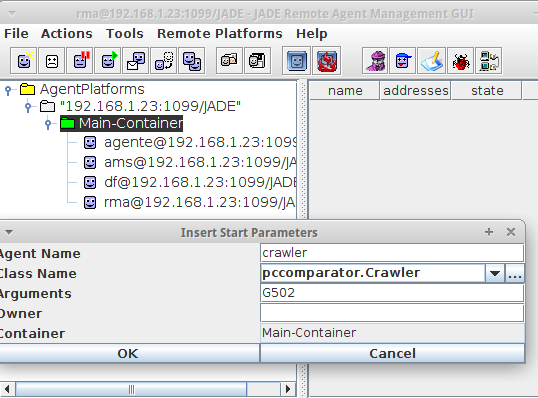
\includegraphics{Captura1}


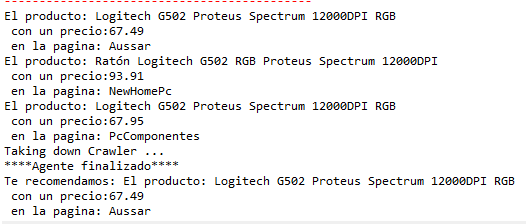
\includegraphics{Captura2}

\end{enumerate}


\end{document}


% Local Variables:
% coding: utf-8
% mode: flyspell
% ispell-local-dictionary: "castellano8"
% mode: latex
% End:
